\documentclass[a4paper]{article}
%\usepackage[singlespacing]{setspace}
\usepackage[onehalfspacing]{setspace}
%\usepackage[doublespacing]{setspace}
\usepackage{geometry} % Required for adjusting page dimensions and margins
\usepackage{amsmath,amsfonts,stmaryrd,amssymb,mathtools,dsfont} % Math packages
\usepackage{tabularx}
\usepackage{colortbl}
\usepackage{listings}
\usepackage{amsmath}
\usepackage{amssymb}
\usepackage{amsthm}
\usepackage{subcaption}
\usepackage{float}
\usepackage[table,xcdraw]{xcolor}
\usepackage{tikz-qtree}
\usepackage{forest}
\usepackage{changepage,titlesec,fancyhdr} % For styling Header and Titles
\usepackage{amsmath}
\pagestyle{fancy}
\usepackage{diagbox}
\usepackage{xfrac}
\usepackage{pgfplots}
\pgfplotsset{compat=1.18}

\usepackage{enumerate} % Custom item numbers for enumerations

\usepackage[ruled]{algorithm2e} % Algorithms

\usepackage[framemethod=tikz]{mdframed} % Allows defining custom boxed/framed environments

\usepackage{listings} % File listings, with syntax highlighting
\lstset{
	basicstyle=\ttfamily, % Typeset listings in monospace font
}

\usepackage[ddmmyyyy]{datetime}


\geometry{
	paper=a4paper, % Paper size, change to letterpaper for US letter size
	top=2.5cm, % Top margin
	bottom=3cm, % Bottom margin
	left=2.5cm, % Left margin
	right=2.5cm, % Right margin
	headheight=25pt, % Header height
	footskip=1.5cm, % Space from the bottom margin to the baseline of the footer
	headsep=1cm, % Space from the top margin to the baseline of the header
	%showframe, % Uncomment to show how the type block is set on the page
}
\lhead{Stochastik für die Informatik\\Wintersemester 2024/2025}
\chead{\bfseries{Übungsblatt 8}\\}
\rhead{Lienkamp, 8128180\\Werner, 7987847}
\begin{document}
\setcounter{section}{8}
\subsection{}
Sei $(X_n)_{n\in N}$ eine Folge von unabhängigen, identisch verteilten Zufallsvariablen mit Dichte\\\\
\(f_{X1}(x) = 
\begin{cases}
    2x, & \text{falls } x \in [0,1],\\
    0, & \text{sonst.}
\end{cases}\)\\\\
Berechnen Sie \(\lim\limits_{n\to\infty}\frac{1}{n}\sum\limits^n_{i=1}X_i\).\\\\
Gleichverteilung der Zufallsvariablen:\\
\(\lim\limits_{n\to\infty} \frac{1}{n}\sum\limits^n_{i=1} X_y = \lim\limits_{n\to\infty} \mathbb{E}[X_i]=\mathbb{E}[X_1]\)\\\\
\(\int\limits^1_0 t\cdot f(t)\, dt = \int\limits^1_0 t\cdot t ^2\, dt = 2 \int\limits^1_0 t^2\, dt = 2 \left[\frac{t^3}{3}\right]^1_0 = 2 \left(\frac{1^3}{3}-\frac{0^3}{3}\right)=\frac{2}{3}\)\\\\
\(\Rightarrow \lim\limits_{n\to\infty}\frac{1}{n}\sum\limits^n_{i=1}X_i=\frac{2}{3}\)
\subsection{}
Sei $X$ eine Zufallsvariablen mit der Dichte\\\\
\(F_X(x)=\begin{cases}
    cxe^{-\lambda x} & \text{falls } x \geq 0\\
    0 & \text{sonst}
\end{cases}\)\\\\
wobei $\lambda > 0$ fest gewählt ist und $c \in \mathbb{R}$ eine geeignete Konstante.\\\\
(a) Bestimmen Sie $c$.\\\\
\(\int\limits^\infty_{-\infty} f_X(t)\, dt \rightarrow \int u\cdot v' = u\cdot v - \int u' \cdot v = c \cdot \left[t\cdot \left(-\frac{1}{\lambda}\right)e^{-\lambda t} - \int 1 \cdot \left(-\frac{1}{\lambda}\right)e^{-\lambda t}\right]^\infty_0\)\\
\(c \cdot \left[-\frac{t}{\lambda}\, e^{-\lambda t}-\frac{1}{\lambda^2}\, e^{-\lambda t}\right]^\infty_0=c\cdot \left(0-0-\left(0-\frac{1}{\lambda^2}\right)\right)=\frac{c}{\lambda^2}\)\\\\
Für die Dichte einer Zufallsvariable muss gelten: \(\frac{c}{\lambda^2}=1 \Rightarrow c = \lambda^2\) \\\\
(b) Berechnen Sie $\mathbb{E}[X]$ und $\mathbb{V}(X)$.\\\\
Aus der Vorlesung kennen wir:\\
$\mathbb{E}[X] = \int\limits_{-\infty}^{\infty} t \cdot f_x(t) dt$.\\
Außerdem ist $f_X(t) = \frac{d}{dt} \cdot F_X(t)$\\
Somit ist $\mathbb{E}[X] = \int\limits_{-\infty}^{\infty} t \cdot \frac{d}{dt} \cdot F_X(t) dt$\\
Diesen Term können wir nun durch partielle Integration vereinfachen Wir definieren: $u = t$, $du = dt$, $dv = \frac{d}{dt} \cdot F_X(t)dt$ und $v = F_X(t)$\\
Die Formel der Partiellen Integration lautet: $\int u dv = uv - \int v du$
Wir wenden dies auf den Ausgangsterm an:\\
$\mathbb{E}[X] = [tF_X(t)]_{-\infty}^\infty - \int\limits_{-\infty}^\infty t F_X(t) dt$\\
Den Term $[tF_X(t)]_{-\infty}^\infty$ können wir eliminieren, weil für die beiden Randwerte bei $\lambda > 0$ für $t \rightarrow \infty$ geht $F_X(t) \rightarrow 0$ (wir nehmen an, dass $\mathbb{E}[X]$ für große $t$ nicht divergiert) und für $t \rightarrow 0$ geht $F_X(t) \rightarrow 0$. $t \rightarrow - \infty$ ist $0$ laut der Definition von $F_X(x)$ für $x < 0 \rightarrow 0$\\
Somit bleibt: $\mathbb{E}[X] = - \int\limits_0^\infty t F_X(t) dt$\\
Die Funktion einsetzen:\\
$\mathbb{E}[X] = - \int\limits_0^\infty t \lambda^2te^{-\lambda t} dt$\\
$\mathbb{E}[X] = - \int\limits_0^\infty \lambda^2t^2e^{-\lambda t} dt$\\
$\mathbb{E}[X] = - \lambda^2 \cdot \int\limits_0^\infty t^2e^{-\lambda t} dt$\\
Zum lösen dieses Integrals kann eine einfache Formel verwendet werden: $\int\limits_0^\infty t^ne^{-\lambda t} dt = \frac{!n}{\lambda^{n + 1}}$\\
$\Rightarrow \mathbb{E}[X] = - \lambda^2 \cdot \frac{!2}{\lambda^{2 + 1}} = - \frac{2}{\lambda}$\\
Nun berechnen wir noch $\mathbb{V}[X] = \mathbb{E}[X^2] - \mathbb{E}[X]^2$\\
$\mathbb{E}[X^2] = - \int\limits_0^\infty t^2 F_X(t) dt$\\
$\mathbb{E}[X] = - \int\limits_0^\infty t^2 \lambda^2te^{-\lambda t} dt$\\
$\mathbb{E}[X] = - \int\limits_0^\infty \lambda^2t^3e^{-\lambda t} dt$\\
$\Rightarrow \mathbb{E}[X] = - \lambda^2 \cdot \frac{!3}{\lambda^{3 + 1}}= - \frac{\lambda^2 \cdot 6}{\lambda^{3 + 1}} = - \frac{6}{\lambda^2}$\\
$\Rightarrow \mathbb{V}[X] = \mathbb{E}[X^2] - \mathbb{E}[X]^2 = - \frac{6}{\lambda^2} - \left(- \frac{2}{\lambda}\right) = - \frac{6 \cdot \lambda}{\lambda^2 \cdot \lambda} + \frac{2 \cdot \lambda^2}{\lambda \cdot \lambda^2} = - \frac{6 \cdot \lambda + 2 \cdot \lambda^2}{\lambda^3} = \frac{2 \cdot (x + 3)}{x^2}$
\\\\
(c) Berechnen Sie die Verteilungsfunktion $F_X$ und skizzieren Sie sie für $\lambda = 2$.\\\\
\(F_X(t) = \int\limits^x_{-\infty} f_X(t)\, dt\)\\\\
aus (a): \(c \cdot \left[-\frac{t}{\lambda}\, e^{-\lambda t} - \frac{1}{\lambda^2}\, e^{-\lambda t}\right]^x_0 = \lambda^2 \cdot \left[-\frac{t}{\lambda}\, e^{-\lambda t}-\frac{1}{\lambda^2}\, e^{-\lambda t}\right]^x_0=\left[-\lambda\cdot te^{-\lambda t} - e^{\lambda t}\right]^x_0\)\\\\
Aufgrund der Exponentialverteilung wissen wir: \(\left[-\lambda \cdot te^{-\lambda t} - e^{\lambda t}\right]^x_0 = 1 - \lambda xe^{-\lambda x} - e^{-\lambda x}\)\\\\
für \(\lambda = 2 \Rightarrow 1 - 2 \cdot xe^{-2x}-e^{-2x}\)\\\\
\begin{tikzpicture}
    \begin{axis}[
        width=10cm, % Breite des Plots
        height=6cm, % Höhe des Plots
        xmin=-1, xmax=5, % Bereich der x-Achse
        ymin=0, ymax=1.2, % Bereich der y-Achse
        xlabel={$x$}, % Beschriftung x-Achse
        ylabel={$y$}, % Beschriftung y-Achse
        axis lines=middle, % Achsen durch den Ursprung
        domain=-1:5, % Bereich für die Funktion
        samples=200, % Anzahl der Punkte
    ]
        \addplot[
            blue, % Farbe der Linie
            thick % Dicke der Linie
        ]
        {1 - 2*exp(-2*x) - exp(-2*x)};
        \legend{$y = 1 - 2e^{-2x} - e^{-2x}$} % Legende
    \end{axis}
\end{tikzpicture}
\subsection{}
Die Verteilung der Zufallsvariable $Z$ ist wie folgt definiert. Eine faire Münze werde geworfen, und falls die Münze Kopf zeigt, sei $Z$ gleichverteilt auf $[1,3]$, sonst sei $Z$ gleichverteilt auf $[2,4]$.\\\\
(a) Berechnen Sie die Verteilungsfunktion $F_Z$ und die Dichte $f_Z$ von $Z$ und skizzieren Sie diese.\\\\
\textbf{Verteilungsfunktion:}\\\\
Es ist gegeben:\\\\
\(\mathcal{B}\sim Ber\left(\frac{1}{2}\right), X\sim \mathcal{U}([1,3]), Y \sim \mathcal{U}([2,4])\)\\
$X$ und $Y$ sind voneinander unabhängig.\\
\(Z=\mathcal{B}X + (1-\mathcal{B})Y\)\\
\(F_Z(x)=\mathbb{P}(Z\leq x \vert \mathcal{B}=0)\cdot \mathbb{P}(\mathcal{B}=0)+\mathbb{P}(Z\leq x \vert \mathcal{B}=1)\cdot \mathbb{P}(\mathcal{B}=1)\\
\hspace*{.85cm}\Rightarrow\mathbb{P}(X\leq x)\cdot \mathbb{P}(\mathcal{B}=1) + \mathbb{P}(Y\leq x) \cdot \mathbb{P}(\mathcal{B}=1)\)\\\\
\(F_Z(x)= 
\begin{cases}
    \mathbb{P}(X<1)\cdot\mathbb{P}(\mathcal{B}=0)+\mathbb{P}(Y<1)\cdot \mathbb{P}(\mathcal{B}=1) = 0\cdot \frac{1}{2}+0\cdot \frac{1}{2}=0 & \text{falls } x<1\\
    \mathbb{P}(X<2)\cdot\mathbb{P}(\mathcal{B}=0)+\mathbb{P}(Y<2)\cdot \mathbb{P}(\mathcal{B}=1) = \frac{x-1}{2}\cdot \frac{1}{2}+0\cdot \frac{1}{2}=\frac{x-1}{4} & \text{falls } 1\leq x<2\\
    \mathbb{P}(X<3)\cdot\mathbb{P}(\mathcal{B}=0)+\mathbb{P}(Y<3)\cdot \mathbb{P}(\mathcal{B}=1) = \frac{x-1}{2}\cdot \frac{1}{2}+\frac{x-2}{2}\cdot \frac{1}{2}=\frac{2x-3}{4} & \text{falls } x2\leq x < 3\\
    \mathbb{P}(X<4)\cdot\mathbb{P}(\mathcal{B}=0)+\mathbb{P}(Y<4)\cdot \mathbb{P}(\mathcal{B}=1) = \frac{1}{2} + \frac{x-2}{2}\cdot \frac{1}{2}+ \frac{x-2}{2}\cdot \frac{1}{2}=\frac{x}{4} & \text{falls } 3\leq x < 4\\
    \mathbb{P}(X)\cdot\mathbb{P}(\mathcal{B}=0)+\mathbb{P}(Y)\cdot \mathbb{P}(\mathcal{B}=1) = \frac{1}{2}+ \frac{1}{2}=1 & \text{falls } 4 \leq x\\
\end{cases}\)\\\\\\
Für die Dichte der Funktion berechnen wir die Ableitungen der Verteilungsfunktionen:\\\\
\(f_Z(x)= 
\begin{cases}
    0 & \text{falls } x<1\\
    \frac{1}{4} & \text{falls } 1 \leq x < 2\\
    \frac{1}{2} & \text{falls } 2 \leq x < 3\\
    \frac{1}{4} & \text{falls } 3 \leq x < 4\\
    0 & \text{falls } 4 \leq x\\
\end{cases}\)\\\\\\
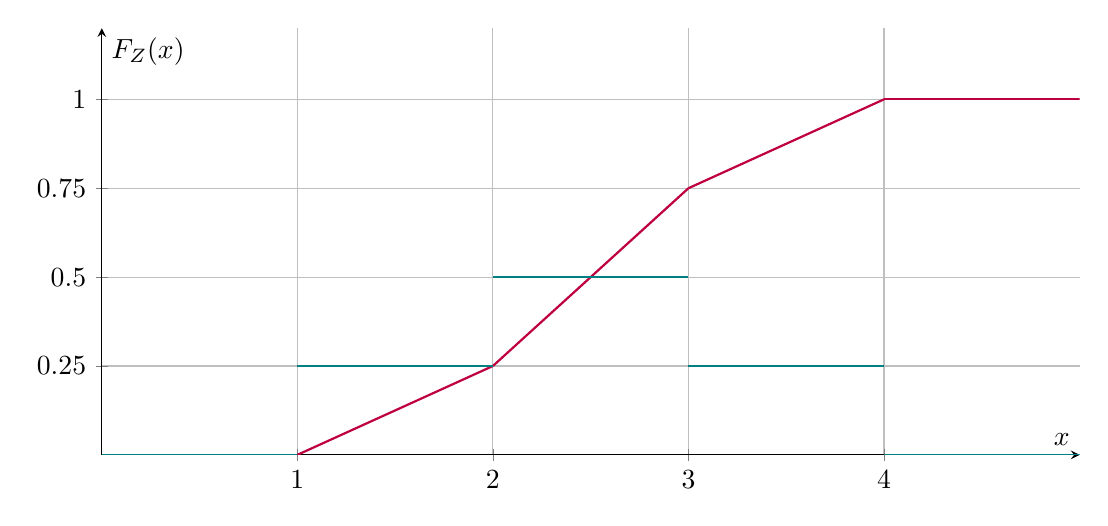
\begin{tikzpicture}
    \begin{axis}[
        axis lines=middle,
        xlabel={$x$},
        ylabel={$F_Z(x)$},
        xmin=0, xmax=5,
        ymin=0, ymax=1.2,
        xtick={1,2,3,4},
        ytick={0,0.25,0.5,0.75,1},
        grid=both,
        width=14cm,
        height=7cm,
    ]
    \addplot[
        domain=0:1, samples=2, thick, color=purple,
    ] {0};
    \addplot[
        domain=1:2, samples=50, thick, color=purple,
    ] {(x-1)/4};
    \addplot[
        domain=2:3, samples=50, thick, color=purple,
    ] {(2*x-3)/4};
    \addplot[
        domain=3:4, samples=50, thick, color=purple,
    ] {(x)/4};
    \addplot[
        domain=4:5, samples=2, thick, color=purple,
    ] {1};
    \addplot[
        domain=0:1, samples=2, thick, color=teal,
    ] {0};
    \addplot[
        domain=1:2, samples=2, thick, color=teal,
    ] {0.25};
    \addplot[
        domain=2:3, samples=2, thick, color=teal,
    ] {0.5};
    \addplot[
        domain=3:4, samples=2, thick, color=teal,
    ] {0.25};
    \addplot[
        domain=4:5, samples=2, thick, color=teal,
    ] {0};
    \end{axis}
\end{tikzpicture}\\\\
\noindent(b) Berechnen Sie $\mathbb{E}[Z^3]$.\\\\
\(\mathbb{E}[Z^3]= \int\limits^4_1 t^3\,f(t)\, dt\)\\
\(\Rightarrow \int\limits^4_1 t^3\, f(t)\, dt = \int\limits^2_1 t^3\, f(t)\, dt + \int\limits^3_2 t^3\, dt + \int\limits^4_3 t^3\, f(t)\, dt = \int\limits^2_1 t^3\, \frac{1}{4}\ dt + \int\limits^3_2 t^3\, \frac{1}{2}\, dt + \int\limits^4_3 t^3\, \frac{1}{4}\, dt\)\\
\(= \frac{1}{4}\int\limits^2_1 t^3\, dt + \frac{1}{2} \int\limits^3_2 t^3\, dt + \frac{1}{4} \int\limits^4_3 t^3\, dt = \frac{1}{4} \left[\frac{t^4}{4}\right]^2_1 + \frac{1}{2}\left[\frac{t^4}{4}\right]^3_2 + \frac{1}{4} \left[\frac{t^4}{4}\right]^4_3\)\\
\(\frac{1}{4}\left(\frac{16}{4}-\frac{1}{4}\right) + \frac{1}{2}\left(\frac{81}{4}-\frac{16}{4}\right)+\frac{1}{4}\left(\frac{256}{4}-\frac{81}{4}\right)= \frac{15}{16}+\frac{65}{8}+\frac{175}{16}= \frac{15}{16}+\frac{130}{16}\frac{175}{16}=\frac{320}{16}=20\)
\subsection{}
Die Dauer $T$ der Reparatur einer Maschine sei exponentialverteilt zum Parameter $\lambda$.\\\\
(a) Wie groß ist die Wahrscheinlichkeit, dass die Reparatur länger als $t > 0$ Zeiteinheiten dauert? Wie groß ist die Wahrscheinlichkeit, dass sie länger als $t$ Zeiteinheiten dauert, wenn sie bereits $s\in(0,t)$ Zeiteinheiten andauert, und noch nicht beendet ist? Was können Sie über die Verteilung Restdauer der Reparatur sagen?\\\\
Wir wissen \(\mathbb{P}(T>t)=\int\limits^\infty_t \lambda e^{-\lambda t}\, dt = \lambda \int\limits^\infty_t e^{\lambda t}\, dt\)\\\\
\textcolor{gray}{NR: \(z = -\lambda t \Leftrightarrow \frac{dz}{dt} = -\lambda \Leftrightarrow dt = \left(-\frac{1}{\lambda}\right)\cdot dz\)}\\\\
\(\Rightarrow \lambda \cdot \int\limits^\infty_t e^z\cdot\left(-\frac{1}{\lambda}\right)\, dz = -\int\limits^\infty_t e^z\, dz = \left[-e^z\right]^\infty_t = \left[-e^{-\lambda t}\right]^\infty_t\)\\\\
\textcolor{gray}{NR: \(\lim\limits_{t\to\infty} -e^{-\lambda t} = \lim\limits_{t\to\infty} \frac{1}{e^{\lambda t}}=0\)}\\\\
\(\Rightarrow 0 - \left(-e^{-\lambda t}\right)=e^{-\lambda t}\)\\\\\\
Für \(\mathbb{P}(T>t \vert T>s)\) ist gegeben \(s\in (0,t)\), es gilt also \(t>s\).\\\\
\(\mathbb{P}(T>t \vert T>s)=\frac{\mathbb{P}(T>t,T>s)}{\mathbb{P}(T>s)}=\frac{\mathbb{P}(T>t)}{\mathbb{P}(T>s)}=\frac{e^{-\lambda t}}{e^{-\lambda s}}=e^{-\lambda (t-s)}\)\\\\
$s=$ vergangene Zeiteinheiten der Reparatur\\
$t=$ insg. Zeiteinheiten der Reparatur\\
\(r= t-s \Rightarrow t=r+s \Rightarrow e^{-\lambda r}\)\\\\
Die Restdauer ist exponentiell mit Parameter $\lambda$ verteilt.\\\\
(b) Berechnen Sie $\mathbb{E}[T\vert T >s]$ für $s>0$.\\\\
Aus a) ist gegeben $r = t - s$\\
$\Rightarrow F_{T|T>s}(t) = 1 - e^{-\lambda r} = 1 - e^{-\lambda (t - s)}$ für $t > s$, also\\
\(
f_{T|T>s}(t) = \begin{cases}
    \lambda e^{-\lambda (t - s)} & \text{falls } t > s\\
    0 & \text{sonst}
\end{cases}
\)\\
Somit können wir den Erwartungswert ausrechnen:\\
$\mathbb{E}[X|T>s] = \int\limits_s^\infty t \cdot \lambda e^{-\lambda (t - s)} dt = \lambda \cdot \int\limits_s^\infty te^{-\lambda r} \cdot e^{\lambda s} dt = \lambda e^{\lambda s} \int\limits_s^\infty te^{-\lambda r} dt$
\end{document}
